\documentclass[twocolumn,amsfont,amssymb,amsmath, showpacs,balancelastpage, nofootinbib]{revtex4-1}
\pdfoutput=1

\usepackage{graphicx}
\usepackage{dcolumn}
\usepackage{bm}
\usepackage{amssymb,amsmath,bm}  
\usepackage{color}
\usepackage[colorlinks,linkcolor=red,citecolor=blue,urlcolor=blue ]{hyperref}
\usepackage{multirow}
\usepackage[utf8]{inputenc}
\usepackage{balance}
\usepackage{enumitem}
\usepackage{lipsum}
\newcommand{\nv}{\hat{\bf n}}
\newcommand{\kalo}{Karhunen-Lo\`{e}ve\,}
\newcommand{\jcap}{JCAP}
\newcommand{\mnras}{MNRAS}
\newcommand{\aap}{A\&A}
\newcommand{\aaps}{A\&AS}
\newcommand{\apjs}{ApJS}
\newcommand{\apjl}{ApJL}
\newcommand{\aj}{Astron. Journal}
\newcommand{\pasp}{Publications of the ASP}
\newcommand{\nar}{New Astronomy Review}
\newcommand{\procspie}{Proceedings of the SPIE}
\newcommand{\physrep}{Physics Reports}
\newcommand{\DAM}[1]{{\color{red}{\bf DA: #1}}}

\begin{document}
  \title{Measurement of the Sunyaev-Zel'dovich effect around cosmic voids}
  \author{David Alonso$^1$}\email{david.alonso@physics.ox.ac.uk}
  \author{J. Colin Hill$^2$}
  \author{Renee Hlozek$^3$}
  \author{David N. Spergel$^{4,5}$}
  \affiliation{$^{1}$University of Oxford, Denys Wilkinson Building, Keble Road, Oxford OX1 3RH, UK}
  \affiliation{$^{2}$Department of Astronomy, Columbia University, New York, NY 10027, USA}
  \affiliation{$^{3}$Dunlap Institute for Astronomy and Astrophysics, University of Toronto}
  \affiliation{$^{4}$Center for Computational Astrophysics, Flatiron Institute, 162 5th Avenue, 10010, New York, NY, USA}
  \affiliation{$^{5}$Department of Astrophysical Sciences, Princeton University, Peyton Hall, Princeton NJ 08544-0010, USA}

  \begin{abstract}
    We stack maps of the thermal Sunyaev-Zel'dovich effect produced by the Planck collaboration
    around the centers of cosmic voids defined by the distribution of galaxies in the CMASS sample
    of the Baryon Oscillation Spectroscopic Survey, scaled by the void effective radii. We report
    a first detection of the associated cross-correlation at the $\sim3.4\sigma$ level. We compare
    the measured excess Compton-$y$ profile around voids with a model based solely on the spatial
    modulation of halo abundance with environmental density. Scaling this expected profile by an
    overall amplitude $\alpha_v$, we find a best-fit value $\alpha_v=0.67\pm0.2$. We discuss
    the possible interpretations of this measurement in terms of modelling uncertainties, excess
    pressure in low-mass halos or non-local heating mechanisms.
  \end{abstract}

  \maketitle

  \section{Introduction}\label{sec:intro}
    \DAM{Introduction: how cool and useful voids are. What the SZ effect is and
         current cool things that have been done with it. The interest
         of measuring the temperature of different environments...}
    
    Throughout this paper we assumed a flat $\Lambda$CDM cosmology with parameters $\Omega_M=0.3$,
    $h=0.7$, $\sigma_8=0.8$, $n_s=0.96$, where $\Omega_M$ is the fractional density of
    non-relativistic species today, $h$ is the normalized expansion rate, $\sigma_8$ is the
    standard deviation of the linear matter overdensity in spheres with a radius of
    $8\,h^{-1}{\rm Mpc}$ and $n_s$ is the primordial spectral index of scalar perturbations. The
    choice of $\Omega_M$ was made to coincide with the value assumed in the construction of the
    void catalog used in this analysis (see Section REF). This was necessary in order to transform
    the comoving lengths used in the catalog into projected angular separations.
    
  \section{The expected void SZ profile}\label{sec:theory}
    The thermal Sunyaev-Zel'dovich effect \cite{1972CoASP...4..173S} traces the hot gas in the
    Universe through the inverse Compton scattering of CMB photons by high-energy electrons.
    This induces a spatial and spectral distortion in the CMB given by
    \begin{equation}
      \frac{\Delta T}{T_{\rm CMB}}=g\left(\frac{h\nu}{kT_{\rm CMB}}\right)\,y(\nv),
    \end{equation}
    where $g(x)=x\,{\rm coth}(x/2)-4$, $y$ is the so-called Compton-$y$ parameter (see below)
    and we have neglected all relativistic corrections.
  
    The Compton-$y$ parameter associated to a particular structure at redshift $z$ is given by
    \begin{equation}\label{eq:sz_main}
      y(\theta)=\frac{\sigma_T}{m_e\,c^2}\int\frac{dr_\parallel}{1+z}P_e
      \left(\sqrt{r_\parallel^2+r_\perp^2}\right),
    \end{equation}
    where $\sigma_T$ and $m_e$ are the Thomson scattering cross section and the electron mass,
    $P_e(r)$ is the electron pressure profile of the structure, $r_\parallel$ and $r_\perp\equiv
    \chi(z)\theta$ are the longitudinal (parallel to the line of sight) and transverse comoving
    distances from the structure, $\chi(z)$ is the comoving distance to redshift $z$ and $\theta$
    is the angular separation from the center of the projected structure.
    
    The tSZ signal around voids can therefore be predicted by estimating their expected excess
    electron pressure profile. This is directly connected to the problem of modelling the
    mechanisms by which baryons are heated in different environments, which has been approached
    from different angles in the literature. One approach is to assume that heating processes
    take place mostly in the dense environments of dark matter halos, and that the gas density and
    temperature can be related to halo mass (e.g. \cite{2001MNRAS.327.1353K} \DAM{add other
    relevant references?}). Under this assumption, the void pressure profile can be directly
    computed in terms of the abundance of haloes of different masses conditional to the
    environmental density given a model for the relation between halo mass and gas density and
    pressure. Such a ``local'' heating mechanism would predict voids to be colder than the
    average, given the under-abundance of massive, hotter halos in underdense environments 
    \cite{1996MNRAS.282..347M}. This description neglects other non-local sources of heating
    of the inter-galactic medium, such as the effect of TeV blazars in the presence of plasma
    instabilities \cite{2012ApJ...752...23C}, which could even give rise to an inverted
    density-temperature relation \cite{2008MNRAS.386.1131B} \DAM{not sure if we should be citing
    other models}.
    
    We do so here by connecting the void density profile, which can
    be estimated directly from the data, with $P_e(r)$ using the so-called ``effective universe''
    approach. This method is spelled out in Appendix \ref{app:effu}, and has been previously used
    in analyses of environmental effects on halo abundances \cite{2003MNRAS.344..715G,
    2004ApJ...605....1G,2009MNRAS.394.2109M,2015MNRAS.447.2683A}). In short, one can
    associate the void underdensity $\delta(r)$ with a set of effective cosmological parameters
    $\Omega_X(r)$, which can then be used to estimate any quantity in the void as its background
    value in that effective cosmology.
    
    The problem therefore reduces to estimating the background free electron pressure for a given
    set of cosmological parameters. Assuming the main contribution to the total tSZ signal comes
    from the hot gas in dark matter haloes, the total electron pressure at a point ${\bf r}$ is
    given by the sum of the contributions from all haloes:
    \begin{align}
      P_e({\bf r})=\int d{\bf x}^3\,dM\,n(M,{\bf x})P_e(|{\bf x}-{\bf r}|,M),
    \end{align}
    where $n(M,{\bf x})$ is the number density of haloes of mass $M$ (i.e. the position-dependent
    halo mass function), with pressure profile $P_e(r,M)$. The background contribution to the
    electron pressure is therefore found by taking the ensemble average of the equation above:
    \begin{equation}\label{eq:pe_bg}
      \langle P_e \rangle=\int dM\,n(M)\frac{4\pi}{3}\int dr\,r^2\,P_e(r,M).
    \end{equation}
    
    To summarize, the process to estimate the void's electron pressure profile is therefore as
    follows:
    \begin{enumerate}
      \item Estimate the void's over-density profile $\delta(r)$.
      \item At a given $r$, relate $\delta(r)$ to a set of effective cosmological parameters
            $\Omega_X(r)$ as described in Appendix \ref{app:effu}.
      \item The void's electron pressure at that $r$ is then computed using Eq. \ref{eq:pe_bg}
            as the background electron pressure for the corresponding effective cosmology
            parameters. Note that, in this equation, both the mass function and the halo
            pressure profile depend on $\Omega_X$.
      \item Integrate the void pressure profile along the line of sight (Eq. \ref{eq:sz_main})
            to obtain the expected tSZ signal.
    \end{enumerate}
    Here we used the estimate of the halo mass function by \cite{2010ApJ...724..878T}, and the
    electron pressure profile of \cite{2012ApJ...758...75B}. The void density profile $\delta(r)$
    was estimated directly from the data in terms of the galaxy overdensity (see Section
    \ref{ssec:results.densprof}). We computed the fiducial $y$ profile used here at a fixed
    redshift $z=0.5$, corresponding to the median redshift of the CMASS sample, and we verified
    that the resulting curve does not vary significantly with $z$ within the allowed redshift
    range. Note that, since all our results are given in terms of the ratio $\theta/\theta_s$,
    where $\theta$ is the angular distance to the void centre and $\theta_v$ is the projected
    void radius, redshift-dependent projection effects are negligible.

  \section{Data}\label{sec:data}
    \subsection{Void catalogs}\label{ssec:data.voids}
      We use the public void catalog described in \cite{2017ApJ...835..161M}, constructed using
      the ZOBOV void finding algorithm \citep{2008MNRAS.386.2101N}, which connects underdensities
      identified through a Voronoi tessellation using a ``watershed'' method. The catalog is based
      on the 12th Data Release of the Baryon Oscillation Spectroscopic Survey (BOSS)
      \cite{2016MNRAS.455.1553R}, part of the Sloan Digital Sky Survey. The full BOSS catalog,
      covering roughly 10,000 ${\rm deg}^2$, is sub-divided into two galaxy samples spanning
      complementary redshift ranges, LOWZ ($\sim4.6\times10^5$ objects, $0.2<z<0.43$) and CMASS
      ($\sim8.5\times10^5$ objects, $0.43<z<0.7$), and void catalogs are provided for both
      samples\footnote{The void catalogs used here
      are available at \url{http://lss.phy.vanderbilt.edu/voids/}.}. Although the authors
      identified more than 10,000 voids in the BOSS dataset, we focused our analysis only on the
      ``cut'' version of the catalogs, in which cuts on significance and minimum density were made
      to ensure a clean sample of underdense regions. In particular we use the CMASS-based catalog,
      containing 774 voids. Each void is assigned an effective radius $r_{\rm v}$ corresponding
      to the radius of the sphere encompassing its Voronoi volume.
      
      For this sample the authors also provide 1,000 mock realizations generated from a set of
      simplified N-body simulations. These mocks are based on a galaxy sample that reproduces
      the clustering properties of the CMASS sample, as well as its angular completeness and
      redshift distribution. As reported by \cite{2017ApJ...835..161M}, the resulting void mock
      catalogs contain on average $\sim20\%$ more voids than the true data, although they
      reproduce statistics of the true void data well in terms of angular, redshift and
      size distribution. We therefore randomly downsampled the mocks to correct for this
      issue. These mocks were used both as randoms to compute the stacked signal around
      the true voids and as ensemble realizations to estimate the measurement uncertainties.
      
      Besides the void catalogs we also made use of the full CMASS galaxy sample, as well as the
      corresponding random catalogues made available by the BOSS collaboration, to estimate the
      average void density profile\footnote{The CMASS data is available at
      \url{https://data.sdss.org/sas/dr12/boss/lss/}}.
      
    \subsection{tSZ and CMB maps}\label{ssec:data.cmb}
      In order to estimate the Sunyaev-Zel'dovich signal associated with voids we make use of
      the Compton-$y$ parameter maps made available by the Planck collaboration
      \cite{2016A&A...594A..22P}. The available maps were derived as linear combinations of
      the Planck High-Frequency Instrument (HFI) intensity maps (100 GHz, 143 GHz, 217 GHz,
      353 GHz, 545 GHz and 857 GHz) smoothed to a common resolution of
      $\theta_{\rm FWHM}=10\,{\rm arcmin}$. The Planck collaboration has released two
      $y$ maps derived using different reconstruction methods: the Modified Internal Linear
      Combination Algorithm (MILCA, \cite{2013A&A...558A.118H}) and the Needlet Internal
      Linear Combination (NILC, \cite{2011MNRAS.410.2481R}). In both cases, the separation
      of the tSZ signal from other sources of emission (CMB and foregrounds) is based mainly
      on its well-known frequency dependence, and both methods find linear combinations of
      the multi-frequency maps that minimize the variance of the resulting map while preserving
      a unit response to the SZ frequency dependence and de-projecting the CMB. The methods
      also use spatial information by constructing independent weights for different scales,
      although they differ in the details of how these weights are derived (see
      \cite{2016A&A...594A..22P}).
      
      There are hints that the NILC is less reliable for the kind of measurement we want to
      make (e.g. \cite{2017MNRAS.467.2315V}), possibly due to its large-scale noise power
      \cite{2016A&A...594A..22P}, which could be difficult to subtract in the absence of
      highly accurate random catalogs. This is especially true in the case of stacking on
      voids subtending relatively large angular scales. For this reason we base our
      analysis on the MILCA $y$ map, although we studied the consistency of our results
      using the NILC map (see Section \ref{ssec:results.syst}).
      
      In order to mitigate the contamination from galactic and extragalactic foregrounds
      we use a combination of the Planck 60\% galactic mask and the union of the HFI and
      LFI point-source masks. In an effort to enhance the signal-to-noise ratio ($S/N$)
      in our measurement, we further mask all SZ sources detected by Planck \cite{2016A&A...594A..27P}
      above $5\sigma$ with redshifts $z<0.43$ (i.e. uncorrelated with the CMASS voids).
      We also make use of the HFI 545 GHz map \cite{2016A&A...594A...1P} to constrain
      the level of foreground and CIB contamination (see Section
      \ref{ssec:results.syst})\footnote{The Planck data is available at
      \url{http://irsa.ipac.caltech.edu/Missions/planck.html}.}.

  \section{Results}\label{sec:results}
    \subsection{The void density profile}\label{ssec:results.densprof}
      Our prediction for the expected void $y$ profile (Section \ref{sec:theory}) requires
      an estimate of the average density profile. The void density profile $\delta(r)$ has
      been the subject of much study in recent years \cite{2002MNRAS.332..205A,
      2014MNRAS.440..601R,2016IAUS..308..542N}, and has been shown to take a fairly universal
      shape across size, redshift and, more importantly, tracer of the underlying density field
      \cite{2014PhRvL.112y1302H,2014MNRAS.442..462S}.
      
      We estimate the void underdensity from the density of tracer galaxies in the CMASS
      sample, using the corresponding random catalog to correct for edge effects and
      incompleteness. For each void $i$ we compute the number of data and random objects
      found in bins of $x=r/r^i_v$, where $r$ is comoving distance from the object to
      the centre of the void and $r_v^i$ is the void's effective radius. The average
      density profile is then estimated as:
      \begin{equation}
        1+\delta_g(x)=\frac{N_R}{N_D}\frac{\sum_i D_i(x=r/r_v^i)}{\sum_i R_i(x=r/r_v^i)},
      \end{equation}
      where $D_i$ and $R_i$ are the histograms of data and random objects found around
      the $i$-th void, $N_D$ and $N_R$ are the total size of the data and random catalogs
      respectively and the index $i$ runs across all the voids in the catalog.
      \begin{figure*}
        \centering
        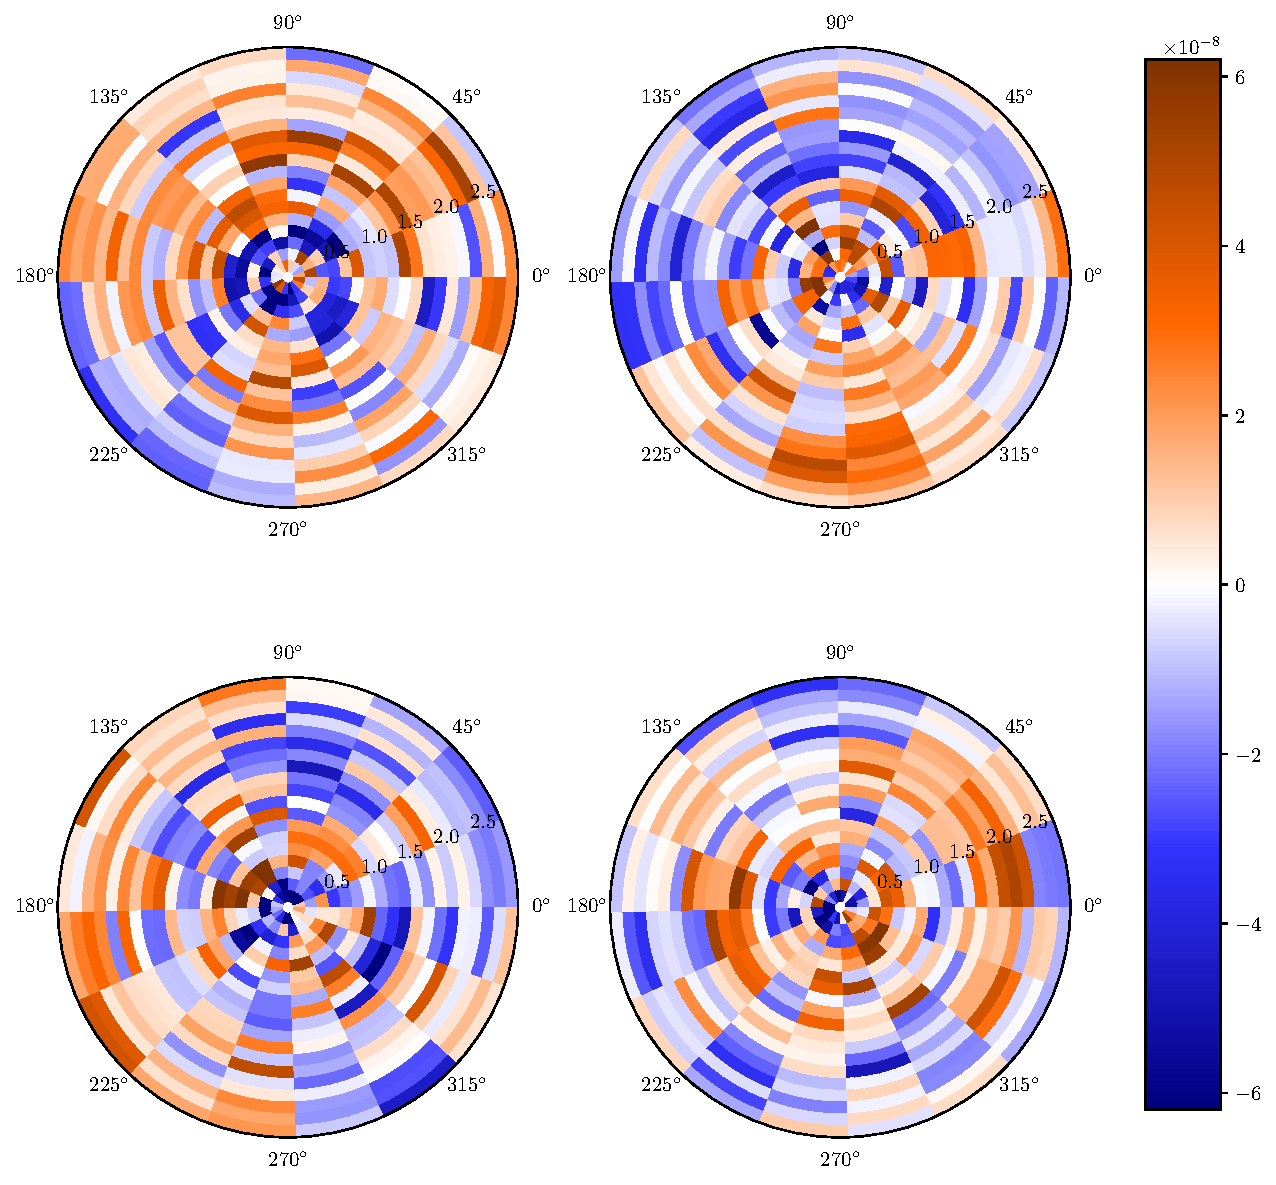
\includegraphics[width=0.9\textwidth]{stacks_2d}
        \caption{2-dimensional stacked tSZ signal in polar coordinates measured around the CMASS voids
                 (top left) and three random mock void catalogues (top right and bottom). The data
                 exhibits a noticeable average decrement below $\theta\lesssim0.7\theta_v$, where
                 $\theta_v$ is the angle subtended by the void effective radius.}
        \label{fig:stacks_2d}
      \end{figure*}
      
      The density profile thus computed corresponds to the underdensity of tracer CMASS
      galaxies around these voids at the median redshift $z\sim0.5$. The effective-universe
      approach, as described in Appendix \ref{app:effu}, is formulated in terms of the
      matter underdensity at redshift $z=0$. To compute this latter quantity in terms
      of $\delta_g(x|z=0.5)$ we must therefore account for the effects of galaxy bias and
      structure growth. To do so we simply rescale $\delta_g$ by a factor
      $[b_{\rm CMASS}D(z=0.5)]^{-1}$, where $b_{\rm CMASS}=2.0$ is the bias of the CMASS
      sample \cite{2013MNRAS.432..743N} and $D(z)$ is the linear growth factor normalized
      at $z=0$. Note that, although in general non-linear contributions to both growth
      and galaxy biasing become important on small scales, recent studies find that this
      problem is alleviated around voids \cite{2017MNRAS.469..787P,2017JCAP...07..014H},
      and this simple linear rescaling should be a good approximation given the uncertainties
      reported here.
      
    \subsection{The SZ signal around voids}\label{ssec:results.yprof}
      \begin{figure}
        \centering
        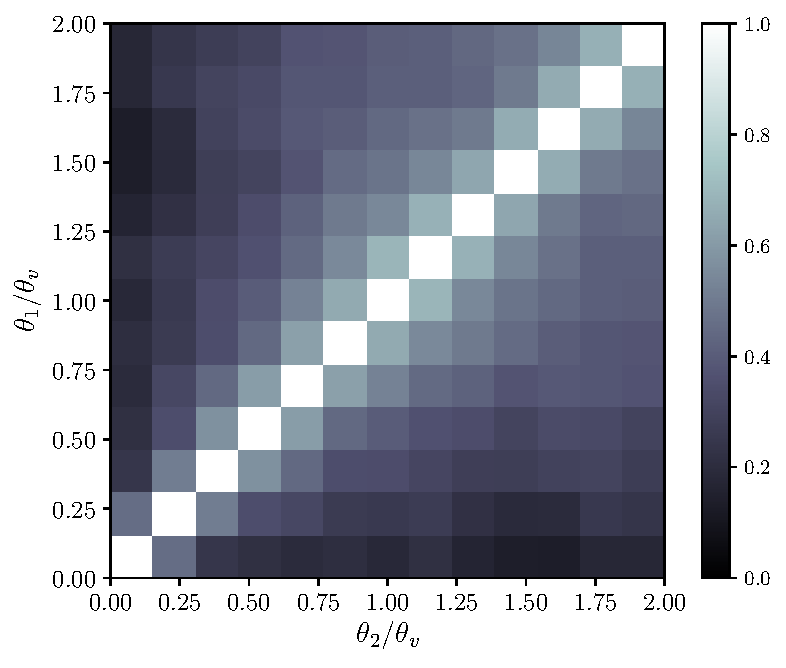
\includegraphics[width=0.49\textwidth]{corrmat}
        \caption{Radial tSZ profile around voids estimated from the CMASS void catalog
                 (red circles with error bars). The dashed black line corresponds to
                 the theoretical expectation based on the model described in Section
                 \ref{sec:theory}, while the black solid line corresponds to the
                 best-fit model found by scaling the fiducial prediction by an
                 amplitude $\alpha_v$.}
        \label{fig:corrmat}
      \end{figure}
      In order to estimate the average tSZ signal around cosmic voids we proceed as follows:
      \begin{enumerate}
        \item For each void $i$ in the catalog, at redshift $z_i$ and with effective radius
              $r^i_v$, we loop over all pixels in the $y$ map lying within a radius
              $3\,\theta^i_v$ of the void's centre, where $\theta^i_v=r^i_v/\chi(z_i)$ is
              the angle subtended by the void's effective radius (here $\chi(z)$ is the
              comoving distance to redshift $z$). For each pixel $p$ we compute two
              quantities: $x_p\equiv \theta_{i,p}/\theta^i_v$ and $\psi_{p}$, where
              $\theta_{i,p}$ is the angular separation between the the pixel and void centres,
              and $\psi_{i,p}$ is the angle that this separation vector forms with the great
              circle connecting the pixel with the North Pole.
        \item For each void we then produce two 2-dimensional histograms, $s^i_y(x,\psi)$ and
              $s^i_N(x,\psi)$
              \begin{align}\nonumber
                &s^i_y(x,\psi)=\sum_p \Theta(\psi_p,\psi,\Delta\psi)\Theta(x_p,x,\Delta x)\,y_p
                \\\nonumber
                &s^i_N(x,\psi)=\sum_p \Theta(\psi_p,\psi,\Delta\psi)\Theta(x_p,x,\Delta x),
              \end{align}
              where $y_p$ is the Compton-$y$ measured in pixel $p$, and $\Theta(x_p,x,\Delta x)$
              is a binning operator for a bin centered at $x$ with width $\Delta x$.
              
              We then estimate the average $y$ parameter in the $x$-$\psi$ plane for catalog $c$
              as $\hat{y}_c(x,\psi)\equiv\sum_i s^i_y(x,\psi)/\sum_i s^i_N(x,\psi)$.
        \item We do this for the CMASS void catalog as well as the $N_{\rm m}=1000$ mock
              catalogs, and finally estimate the average tSZ signal corrected for sky coverage
              and completeness by subtracting the mock average:
              \begin{equation}\label{eq:stack_estimator}
                \bar{y}(x,\psi)=\hat{y}_{\rm CMASS}(x,\psi)-
                \frac{1}{N_{\rm m}}\sum_{c=1}^{N_{\rm m}}\hat{y}_c(x,\psi).
              \end{equation}
      \end{enumerate}
      In broad terms, the estimator is therefore a simple stack around voids of the $y$ map in
      polar coordinates scaled by the effective void size. We have not implemented further
      refinements to the method, such as optimally filtering the $y$ map for each void as
      done in e.g. \cite{2017MNRAS.466.3364C}, which might be able to marginally enhance the
      significance of this measurement, in order to facilitate the computation of the associated
      theoretical prediction. In our analysis we computed $\bar{y}(\theta/\theta_v,\psi)$ in
      20 radial bins for $0\leq\theta/\theta_v\leq3$ and 16 angular bins for $0\leq\psi<2\pi$.
      \begin{figure}
        \centering
        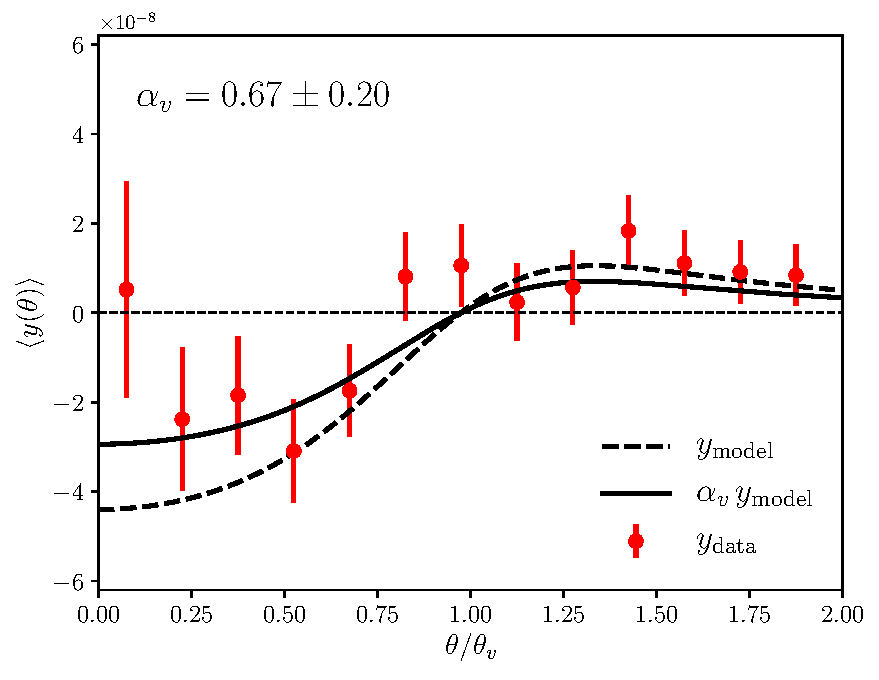
\includegraphics[width=0.49\textwidth]{y_result}
        \caption{Radial tSZ profile around voids estimated from the CMASS void catalog
                 (red circles with error bars). The dashed black line corresponds to
                 the theoretical expectation based on the model described in Section
                 \ref{sec:theory}, while the black solid line corresponds to the
                 best-fit model found by scaling the fiducial prediction by an
                 amplitude $\alpha_v$.}
        \label{fig:y_result}
      \end{figure}
      
      Figure \ref{fig:stacks_2d} shows the stacked SZ signal around voids in polar coordinates
      for the CMASS catalog (upper left) and for three random mocks. Although the measurement
      is noisy, a decrement in $y$ for $x<1$ with respect to the mean can clearly be appreciated
      in the real data.
      
      Although the two-dimensional stacks are useful for visualization purposes, we do not 
      expect a preferred orientation of the void signal, and therefore we proceed by
      considering only the radial tSZ profile (i.e. summing $s_y$ and $s_N$ over $\psi$)
      as our data vector. We further limit the size of this vector to the 13 $x$-bins with
      $x<24$, and write the profile measured in the $k$-th bin as $\bar{y}_k$.
      
      We estimated the covariance matrix of $\bar{y}_k$ from the scatter of the 1000 mock catalogs:
      \begin{equation}
        C_{kk'}=\frac{1}{N_{\rm m}}\sum_{c=1}^{N_{\rm m}}
        \left(\bar{y}^c_k-\langle\bar{y}_k\rangle\right)\,
        \left(\bar{y}^c_k-\langle\bar{y}_k\rangle\right),
      \end{equation}
      where $\bar{y}^c_k$ is the measurement in the $c$-th mock, and $\langle\bar{y}\rangle$ is
      the average across mocks. Figure \ref{fig:corrmat} shows the estimated correlation matrix
      $R_{kk'}\equiv C_{kk'}/\sqrt{C_{kk}C_{k'k'}}$. Note that, because of the beam smoothing
      of the $y$ maps, as well as the mixing of scales caused by the effective rescaling of
      the map with void size, there are significant off-diagonal contributions to the covariance,
      which need to be accounted for.

      In order to quantify the significance of this measurement or the degree of agreement with
      a given model $y^{\rm mod}_k$, we compute the $\chi^2$:
      \begin{equation}
        \chi^2(y^{\rm mod})\equiv\sum_{k,k'}(\bar{y}_k-y^{\rm mod}_k)\,I_{kk'}\,
        (\bar{y}_{k'}-y^{\rm mod}_{k'}),
      \end{equation}
      where $I_{kk'}$ is the inverse covariance matrix. We estimate $I_{kk'}$ as the inverse of
      the sample covariance $C_{kk'}$ corrected for the overall scaling factor prescribed by
      \cite{2007A&A...464..399H}:
      \begin{equation}
        I_{kk'}=\frac{N_{\rm m}-n_d-2}{N_{\rm m}-1}(C^{-1})_{kk'},
      \end{equation}
      where $n_d$ is the size of the data vector. We verified that the distribution of $\chi^2$
      values for the 1000 mock void catalogues for a null model ($y^{\rm mod}=0$, since the
      mocks and $y$ maps are uncorrelated) is well described by a ``chi-squared'' distribution
      with 13 degrees of freedom. Therefore, the $\chi^2$ can be reliably interpreted as the
      likelihood of $y^{\rm mod}$ given the data $\bar{y}_k$.
      
      As a model for the expected tSZ signal in voids we use the theoretical prediction
      described in Section \ref{sec:theory} and scaled by an amplitude $\alpha_v$ that
      we fit for. Since this is a linear model, the best-fit and standard deviation of
      $\alpha_v$ can be computed analytically as:
      \begin{align}
        \alpha_v&=\frac{\sum_{k,k'}y_k^{\rm mod}I_{kk'}\bar{y}_{k'}}
                            {\sum_{k,k'}y_k^{\rm mod}I_{kk'}y^{\rm mod}_{k'}},\\
        \sigma(\alpha_v)&=\left[\sum_{k,k'}y_k^{\rm mod}I_{kk'}y^{\rm mod}_{k'}\right]^{-1},
      \end{align}
      where here $y^{\rm mod}$ is the theoretical model with a fiducial amplitude
      $\alpha_v^{\rm fid}=1$. Doing this we obtain a best-fit value and uncertainty
      $\alpha_v=0.668\pm0.199$, corresponding to a $\sim3.4\sigma$ measurement of
      the tSZ signal in voids. Figure \ref{fig:y_result} shows the measured signal (red
      circles with error bars), the fiducial theory prediction (dashed black line) and the
      best-fit scaled model (solid black line). The $\chi^2$ for this best-fit model is
      $\chi^2(\alpha_v)=15.3$, corresponding to a probability-to-exceed (PTE) of
      0.22 for 12 degrees of freedom. In contrast, for the null model we obtain 
      $\chi^2({\rm null})=26.6$, with a PTE of 0.012. The significance of this measurement
      in terms of a $\chi^2$-difference is therefore $\sqrt{\Delta\chi^2}=3.36$, in
      agreement with our previous estimate.
      
    \subsection{Null tests and systematics}\label{ssec:results.syst}
      In order to test the robustness of this measurement, we have studied the possible
      impact of certain systematic uncertainties and performed a number of consistency tests.
      \begin{figure}
        \centering
        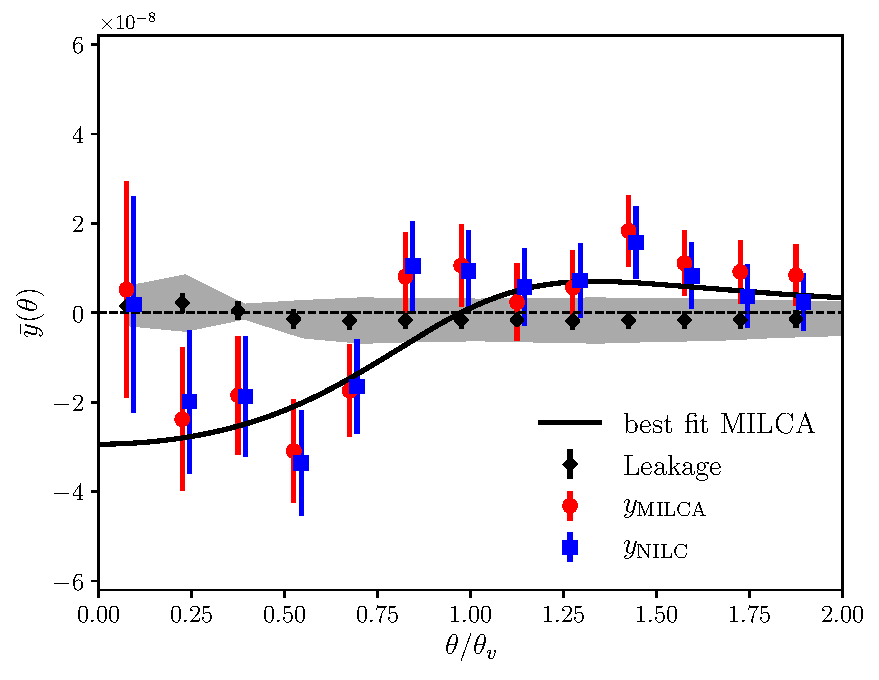
\includegraphics[width=0.49\textwidth]{y_syst}
        \caption{Radial tSZ profile around voids estimated from the CMASS void catalog
                 (red circles with error bars). The dashed black line corresponds to
                 the theoretical expectation based on the model described in Section
                 \ref{sec:theory}, while the black solid line corresponds to the
                 best-fit model found by scaling the fiducial prediction by an
                 amplitude $\alpha_v$.}
        \label{fig:y_syst}
      \end{figure}
      
      A first simple test for the presence of systematic errors is cross-correlating the
      CMASS voids with the ``half-difference'' Compton $y$ map, constructed by differencing
      the $y$ maps constructed using the first and second halves of stable pointing periods,
      and distributed together with the full MILCA map. The half-difference map should
      therefore contain only noise and no real $y$ signal. We carried out the same analysis
      described in Section \ref{ssec:results.yprof} on this half-difference map, including
      the computation of the associated covariance matrix, and find that the signal measured
      from the data is compatible with zero, with a $\chi^2=12.8$ (${\rm PTE}=0.464$).
      
      We have also studied the consistency of our measurement by repeating it on the NILC
      Compton-$y$ map. We find that the measured void $y$ profile agrees with the
      measurement from the MILCA map up to an overall additive offset. As mentioned in
      Section \ref{ssec:data.cmb} and pointed out by \cite{2017MNRAS.467.2315V}, the NILC
      map suffers from a higher large-scale noise power than the MILCA (see e.g. Fig. 5 of
      \cite{2016A&A...594A..22P}). This large-scale contribution, as well as the overall
      amplitude of the void signal, are much smaller ($\sim O(10^{-8})$) than the typical
      per-pixel noise ($\sim O(10^{-6})$). Therefore any imperfection in the removal
      of the mean contribution to the correlation function estimator (i.e. the second term
      on the right hand side of Eq. \ref{eq:stack_estimator}), such as small deviations
      in the BOSS mock void catalogues from the true BOSS footprint, may give rise to an
      overall offset in the estimator. This is particularly relevant for the void stacks,
      given the larger angular scales involved, compared to the usual stacking analyses
      around groups or clusters.
            
      To correct for this issue, we introduce an extra free parameter in our model,
      corresponding to an overall additive amplitude $\alpha_{\rm off}$, and fit for it
      jointly with the amplitude of the void profile $\alpha_v$. The measurement of the
      void $y$ profile in the NILC map corrected for this offset is shown as blue dots
      in Fig. \ref{fig:y_syst}, which also shows the original MILCA measurement in red.
      This procedure yields a measurement of $\alpha_v$ from the NILC map that is in
      agreement with our previous estimate, $\alpha_v= 0.64\pm 0.21$, with a similar
      significance. The measured offset $\alpha_{\rm off}= (1.4\pm 0.5)\times10^{-8}$
      is significant at the $\sim2.8\sigma$ level, and the overall fit is good, with a 
      ${\rm PTE}=0.21$. It is also worth pointing out that, after repeating this analysis
      on the MILCA map, we find that the measured offset is compatible with $0$ in this
      case, and that the recovered value of $\alpha_v$ and its significance does not
      change significantly with respect to the fiducial analysis.
      
      Finally, we quantify the level of contamination of our measurement by other
      potential correlated components. In particular we focus on the contribution from
      imperfectly cleaned dust and CIB emission, which is a known contaminant of the
      Planck $y$ maps \DAM{cites}. To do this, we follow the procedure described in
      \cite{2017MNRAS.467.2315V} and \cite{2014JCAP...02..030H}, making use of the
      Planck 545 GHz map as a tracer of dust. We outline the method here, and we
      refer the reader to these papers for further details.
      
      We start by assuming that the $y$ map is contaminated by CIB and galactic
      emission, such that the observed map is
      \begin{equation}
        y_{\rm obs}=y_{\rm true}+\alpha_{\rm CIB}\,T_{\rm CIB}+\alpha_{\rm gal}T_{\rm gal},
      \end{equation}
      and that the 545 GHz map is dominated by precisely these components
      \begin{equation}
        T_{\rm 545}=T_{\rm CIB}+T_{\rm gal}.
      \end{equation}
      We can then determine the leakage amplitudes $\alpha_{\rm CIB}$ and $\alpha_{\rm gal}$
      by analyzing the auto-correlation of the 545 GHz map and its cross-correlation with
      the observed $y$ map. This also requires the use of existing models for the
      CIB power spectrum and its true cross-correlation with the tSZ signal, for which
      we use the measurements of \cite{2014A&A...571A..30P} and \cite{2016A&A...594A..23P}
      respectively. After masking 80\% of the sky we obtain
      $\alpha_{\rm CIB}=(2.3\pm6.6)\times10^{-7}\,({\rm MJy/sr})^{-1}$ and
      $\alpha_{\rm gal}=(-0.8\pm1.9)\times10^{-7}\,({\rm MJy/sr})^{-1}$.
      
      Since the galactic component should not correlate with the void distribution (unless
      regions of large galactic dust absorption could affect the void finding procedure),
      the most dangerous source of leakage would be the CIB component. The contribution of
      this source of contamination to the measured $y$ void profile, $\bar{y}_{545}$ can
      therefore be quantified by repeating the void stacking measurement on the 545 GHz map and
      scaling the resulting signal, $\bar{T}_{545}$ with $\alpha_{\rm CIB}$:
      $\bar{y}_{545}=\alpha_{\rm CIB}\,\bar{T}_{545}$. The resulting estimated leakage is shown
      as black dots in Figure \ref{fig:y_syst}, with the shaded region corresponding to the 
      level of leakage allowed by the $1\sigma$ uncertainties on $\alpha_{\rm CIB}$.
      \DAM{Discuss more. Say that this agrees with the rough expectation based on naive
      cross-correlation.}

  \section{Discussion}\label{sec:discussion}
    \lipsum[4]

\section*{Acknowledgements}
  The authors would like to thank Nick Battaglia, Adam Lidz and Mark Richardson for useful
  comments and discussions. DA also thanks the Center for Computational Astrophysics, part
  of the Simons Foundation, for their hospitality. DA aknowledges support from the Science
  and Technology Facilities Council and the Leverhume and Beecroft Trusts. \DAM{more?}

\bibliography{paper}

\appendix
%\onecolumngrid
\section{The effective-universe approach to void-related quantities}\label{app:effu}
  It is a well-known result, valid in both Newtonian and relativistic gravitational theory
  (e.g. \cite{1947MNRAS.107..410B}), that a spherically-symmetric overdensity residing
  in an otherwise homogeneous Universe will evolve, at any distance $r$ from its centre, as
  a parallel Friedmann-Lema\^itre-Robertson-Walker universe with effective cosmological
  parameters. These can be related to the density profile $\delta(r)$ and local infall
  velocity of the overdensity (the latter defining the local expansion rate) as:
  \begin{align}
    &\Omega_M(r)=\Omega_M^{\rm BG}\frac{1+\Delta(r)}{\eta^2(r)},\hspace{6pt}
    \Omega_\Lambda(r)=\frac{\Omega_\Lambda^{\rm BG}}{\eta^2(r)},\\
    &H_0(r)=H_0^{\rm BG}\eta(r),
    \hspace{6pt}\Delta(r)\equiv\frac{3}{r^3}\int_0^rds\,s^2\,\delta(s),
  \end{align}
  where $\Delta(r)$ is the average overdensity enclosed within a sphere of radius $r$,
  and all quantities labelled ${\rm BG}$ are the cosmological parameters of the background
  universe. The ratio between expansion rates can be fixed by imposing a homogeneous age
  of the Universe:
  \begin{equation}
    t_{\rm BB}=\frac{1}{H_0}\int_0^1
    \frac{dx}{x\sqrt{\Omega_Mx^{-3}+\Omega_\Lambda+\Omega_Kx^{-2}}},
  \end{equation}
  effectively making the perturbation a purely growing mode that vanishes at early times.
  
  The computation of the background tSZ signal (Eq. \ref{eq:pe_bg}) requires an estimate
  of the halo mass function, which depends on the evolution of both the background and
  linear perturbations. For deep underdensities, the cosmological constant's contribution
  to the total energy density dominates over that of matter, and therefore perturbations
  grow more slowly at late times than in the background cosmology. This effect can be
  taken into account by scaling the value of $\sigma_8$ outside the void by the ratio of
  the linear growth factors in the effective and background cosmologies with the same
  normalization at early times.

\end{document}
